% Chapter Template


\chapter{Theory of Routing Algorithms} % Main chapter title
%----------------------------------------------------------------------------------------
\label{dash7}

\lhead{Chapter 2. \emph{New Routing algorithms in ICN}} % Change X to a consecutive number; this is for the header on each page - perhaps a shortened title

As it is also in IP routing's networks, routing is responsible for building the routing table and maintaining it in face of network changes, including both long-term topology and policy changes as well as short-term churns.  When there is a change in the network, routers need to exchange routing updates with each other in order to reach new global consistency. The time period after a change happens and before all routers agree on the new routing state is called the routing convergence period. Routing protocols need to converge fast in order to reduce packet loss and resume packet delivery after network changes. NDN routing does not need to converge fast thanks to its architecture and needs some strategies to pipline the packets to the destinations.

According to \cite{oran} as we also work on mobility part of ICN: Some ICN designs are extremely mobile friendly, allowing  both  clients  and  servers  to  move  without  needing complex rendezvous techniques as in existing   IP-based approaches explains well why we have designed our algorithms in this vision.

\section{NFD in NDN Networks}
NFD is a network forwarder that implements NDN forwarder. After the initial release, NFD became a core component of the NDN Platform and will follow the same release cycle. 

There are different modules on NFD for different stuffs like \textit{core} which produce different varities between different modules of NFD. \textit{Faces} implements the face concept in NDN. \textit{Tables} which contains some data structures like Content Store (CS) and tables like FIB and PIB for forwarding and pending information for NDN Data/Interest packets and \textit{Forwarding}, which interacts with forwarding strategies to choose and manage faces and \textit{RIB Management} which implements routing table information about routes and each prefix according to propoer faces. this is not a seperate module from NFD Management. Basically we create some faces for each prefix by a given routing strategy which are proposed in this work and it will fill up FIB properly against these information by which you find proper routes.

For example figure \ref{nfd} shows 2 faceIDs which are created by our proposed routing strategies in RIB and FIB: $67344$, $67876$. As you see these faces have routes toward 'jordan' and 'luca' thanks to strategies of TreeOnProducer.   

As you can see also in this figure there are different Forwarding strategies for different namespaces. We also added an option on Lurch to change it on run time.



\begin{figure}[H]

\begin{center}

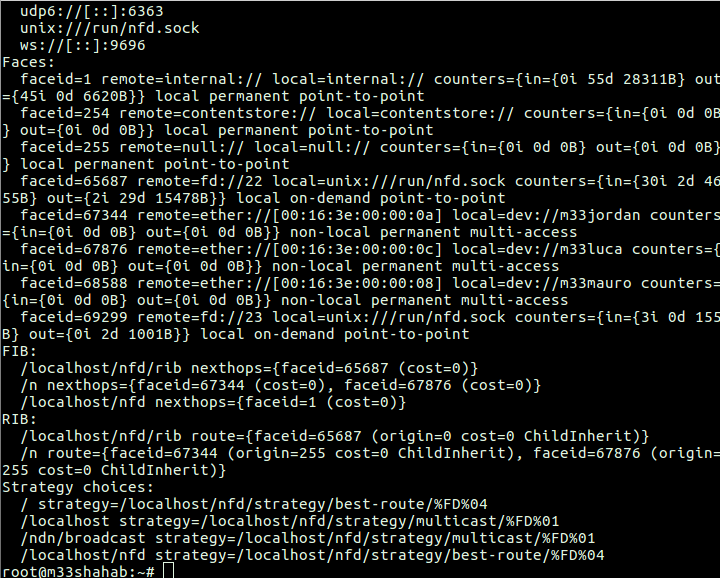
\includegraphics[scale = 0.35]{Pictures/nfd.png}

\caption{nfd-status on shahab container} \label{nfd} 

\end{center}

\end{figure}


Picture \ref{nfd} shows well that there is no route for 68588 in RIB which means as \cite{jacobson} also says forwarder engine needs a Software to do this kinds of selection which explains very well the reason why we work on these strategies. Each forwarder must decides this selection using proper strategy. 

%----------------------------------------------------------------------------------------
%	SECTION 1
%----------------------------------------------------------------------------------------
\section{Routing in NDN}
In NDN, the forwarding plane is the actual control plane
since the forwarding strategy module makes forwarding decisions on its own.  This fundamental change prompts us
to rethink the role of routing in NDN. Routing protocols are responsible for disseminating topology and policy information, computing routes and handling short-term network changes.

\textit{Shortest path}, \textit{Distance Vector}, \textit{Link state} and their variants IS-IS and OSPF are the routing algorithms that are most widely used inside large networks and the Internet of today from ARPANET (Bellman, 1957; and Ford and Fulkerson, 1962). (\cite{modulation})


 
\section{Routing Strategies}
\textit{ShortestPath} and \textit{Djikstra} algorithms are designed to obtain the paths which minimizes the cost metric of each link. 

In this subsection we introduce 4 different algorithms which are defined in function of network's need for NDN networks.

We will also mention the ideas and reseaons for these strategies. Next section we will show some results and figures about algorithms for one medium size and large size of network.

In this work we will work on Shortest path using different metrics. Basically number of hops for links in order to calculate our routes properly in function of network postion.

\textit{ShortestPath} In \textit{Networkx} Python library is called \textit{Unweighted} method for Graph becasue it assumes number $1$ for each link which is simply number of hops. In ndnSim which is an ndn simulator, this weight has been put $1$ because of NDN. In this library \textit{Djikstra} is called \textit{weighted} methods becasue it cares about the number of weight to which the link is mapped and it's the way how it obtains proper paths. 

For Discovering more about algorithms we refere you to \ref{Appendix} to see the details of implementation. 

\subsection{Consumer $\&$ Producer Trees Strategy}
In ICN the cost metric is \textit{number of hops} becasue of naturity of ICN architecture in which you \textit{search} content so basically in Graph sense nearer nodes are preferred always. This is the idea that enables us to think about \textit{TreeOnConsumer} and \textit{TreeOnProducer} strategies in which you want to find the tree which finds the shortest paths either from one producer to consumers or one consumer to producers properly.

The idea of \textit{TreeOnConsumer} is based on this concept that imagine once in cellular networks at the same time maybe you can have $N$ clients or consumers that searche exactly the same \textit{content}, like a special video.

Figure \ref{consumer} shows this concept properly.


\begin{figure}[H]

\begin{center}

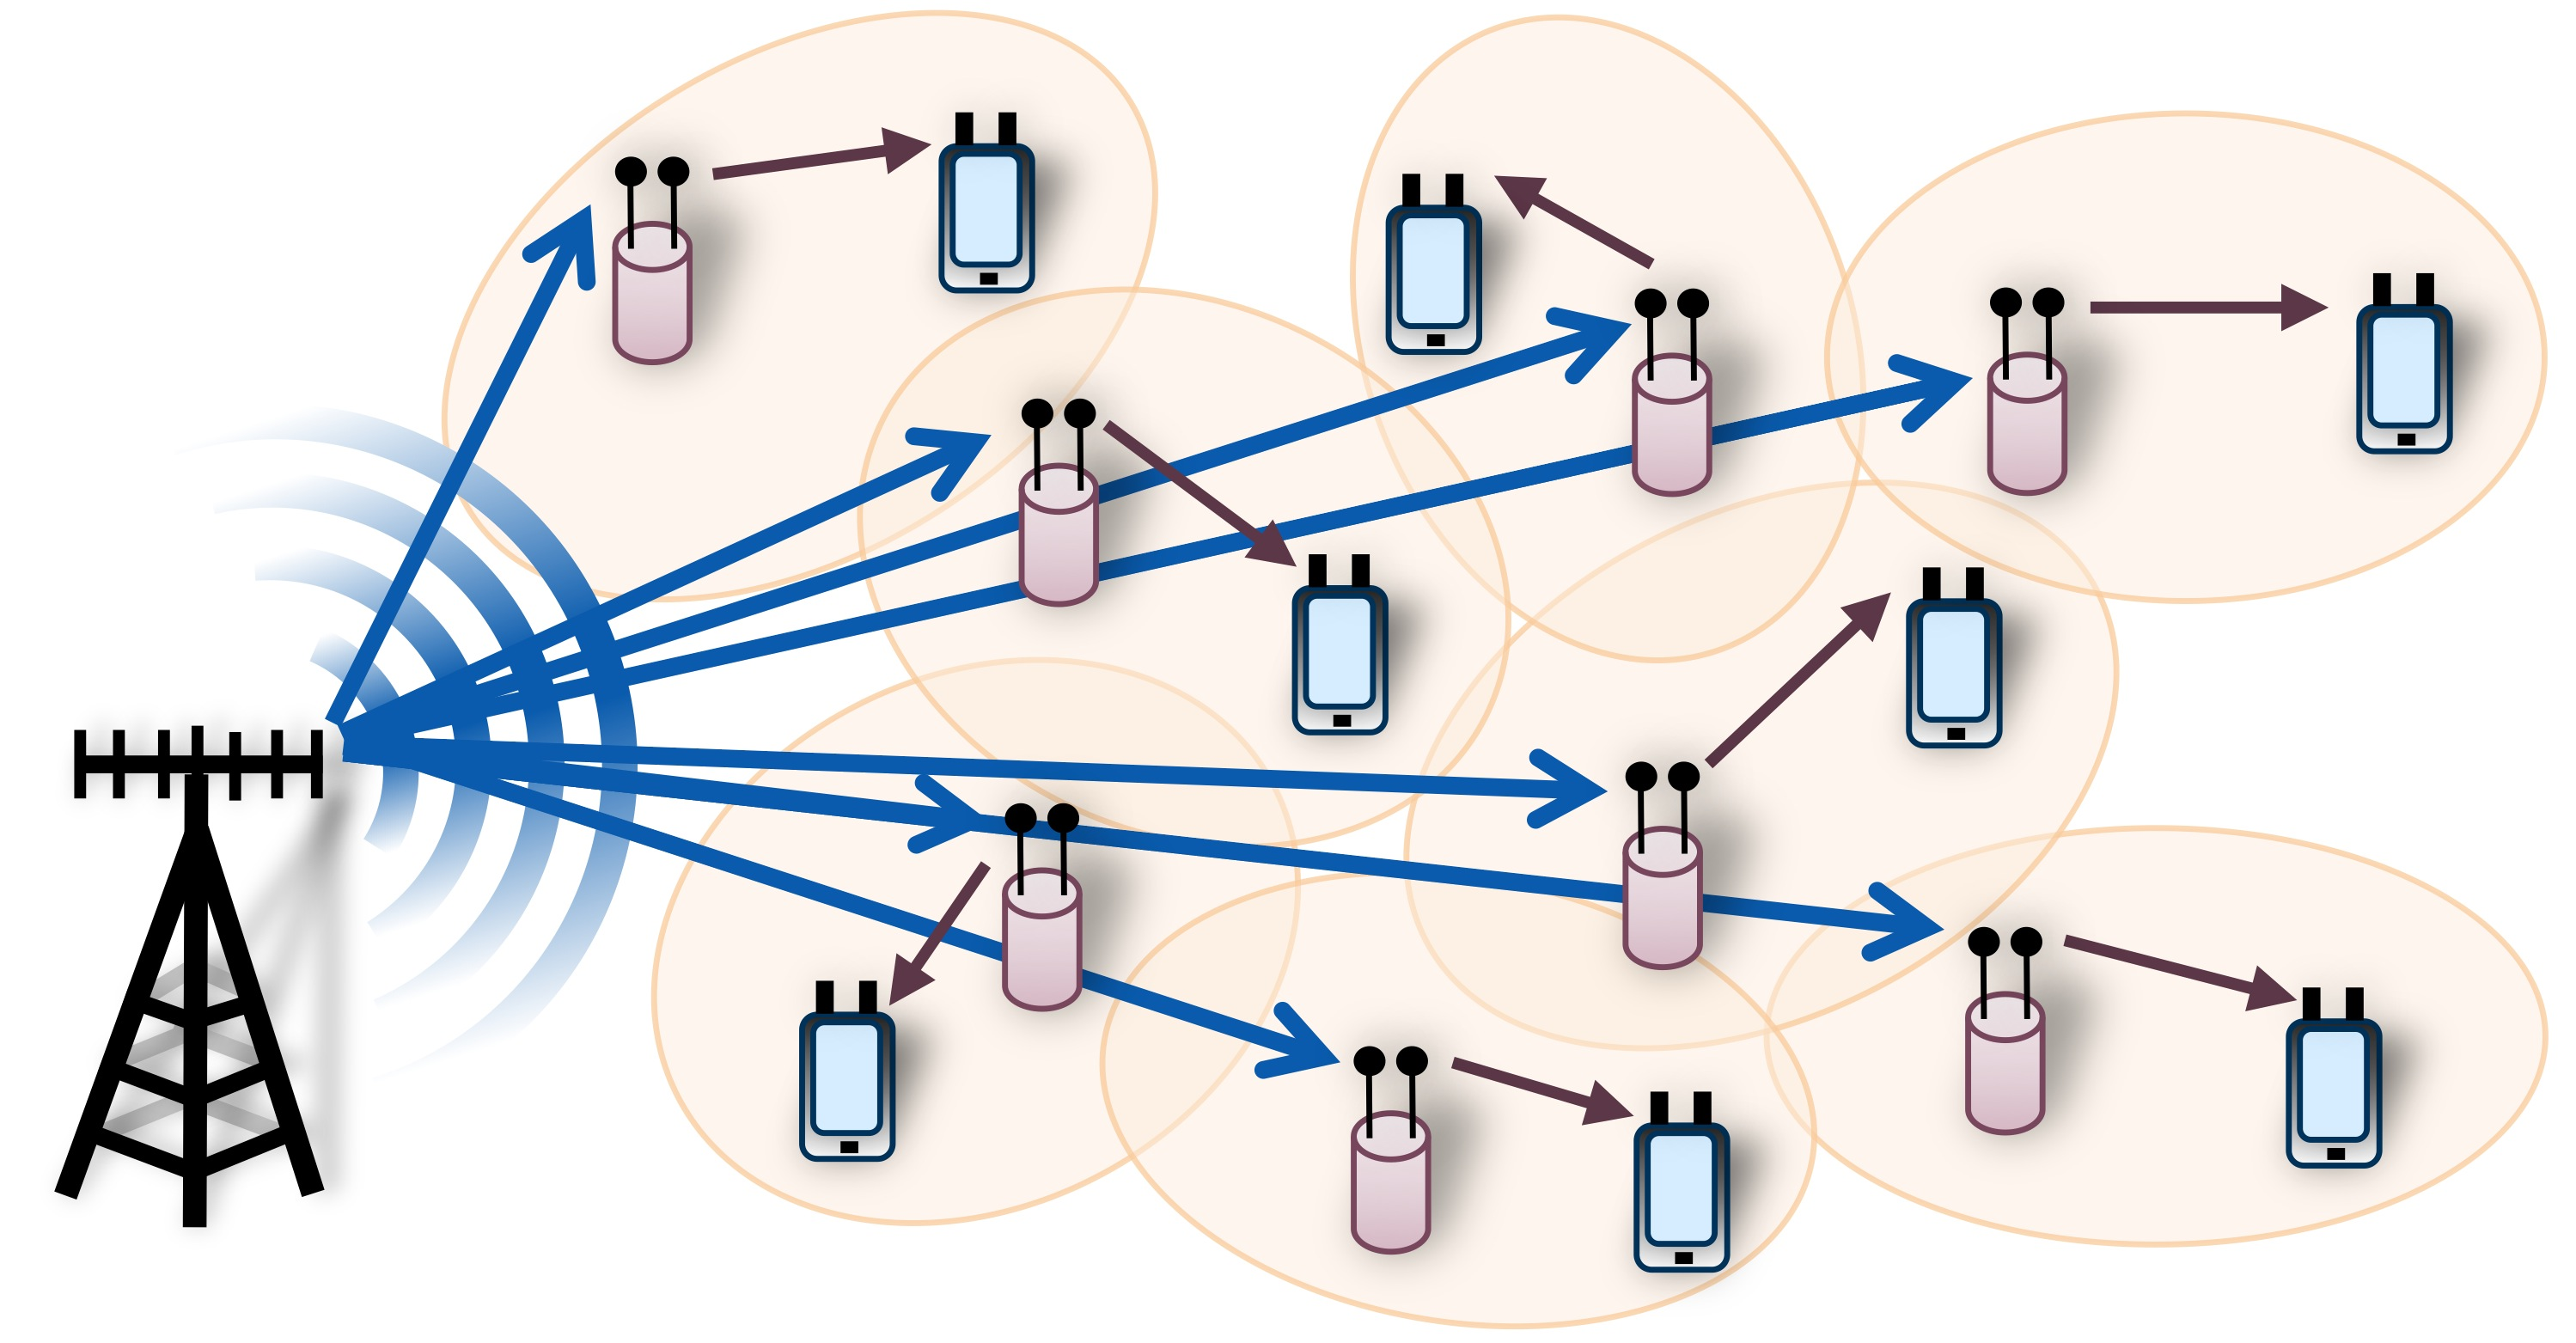
\includegraphics[scale = 0.1]{Pictures/treeonconsumer.jpg}

\caption{TreeOnConsumer} \label{consumer} 

\end{center}

\end{figure}
     

\textit{TreeOnProducer} is a bit inverse thinking of previous algorithm, in which imagine you, as a client to speed up your video downloading you can retrive your data using different repositories packets to catch up (Figure \ref{producer}).

\begin{figure}[H]

\begin{center}

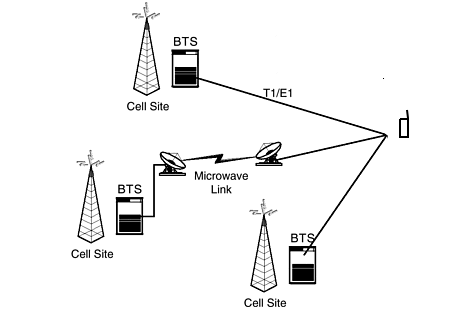
\includegraphics[scale = 0.4]{Pictures/treeonproducer.png}

\caption{TreeOnProducer} \label{producer} 

\end{center}

\end{figure}


\subsection{Minimum Cost MultiPath Strategy}
Imagine a case you have multiDestination, like a live videostreaming football match that has a lot of viewers in the network at the same time, in this case nodes should do some kind of multicast sending packets to the networks so network should choose the routes which minimizes the cost of links from source to destinations. The cost is always number of hops in ICN context because of naturity of architecture. 

Figure \ref{balance} shows well the idea of this strategy which is designed for multi-destination case with minimizing cost.

\begin{figure}[H]

\begin{center}

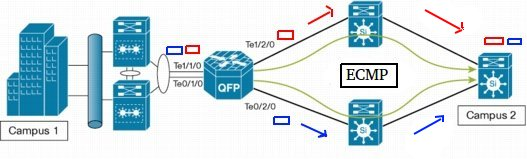
\includegraphics[scale = 0.7]{Pictures/balance.jpg}

\caption{Eqaul Cost Multipath Strategy on CISCO Router} \label{balance} 

\end{center}

\end{figure}

As you can see in \ref{balance} is a simple topology example of real cisco routers implemented between 2 campus in this case you can deliver packets, one by one wich means packets can travers through one upper path and the other with belower path.

\textbf{Multi-Producer, Multi-Consumer} is when you have multiple consumers who are searching the same content and multiple producers for this content. This algorithm is the core of the strategies becasue of its ability. Actually this algorithm looks at the position of clients and producers then for each client finds the closest producer (as we said number of hops is always our metric) then routing is done.



\subsection{Maximum Flow Strategy}
This strategy is done by calculation of paths and links which produce maximum throughput from source node to sink node. \textit{MaxFlow} is very important strategy which allows the links to participate in subgraph which maximizes the capacity and basically it creates an one-directed graph and all ratio traffic through these links should be calculated by this strategy. Figure \ref{max} shows well this explanation. Algorithm has chosen paths which maximizes flow to the sink node.

\begin{figure}[H]

\begin{center}

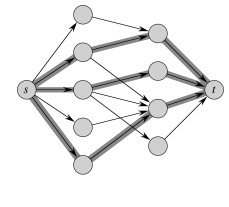
\includegraphics[scale = 0.8]{Pictures/max.jpg}

\caption{Maximum Flow Strategy} \label{max} 

\end{center}

\end{figure}


 
Specially this strategy can be used when mobile phones want download video packets with very high quality video coding rates (i.e Ultra HD ,4K, ...) or to speed up downloading content and the network allows to get information through different paths from sources to clients. This strategy works with a weight (\textit{capacity}) on each link.

As it's clear there is some paths which are not selected becasue it wouldn't produce total maximum flow on network.  The idea of this strategy is to use throughput capability of network to achieve to have the best quality at the edge user experience. 







